\documentclass[12pt,a4paper]{article}
\usepackage{pgf}
% \usepackage[condensed,math]{kurier}
% \usepackage[T1]{fontenc}
\usepackage{svg}
\usepackage{tikz}
\usepackage{stanli}
\usepackage{afterpage}
\usepackage{multirow}
\usepackage{subfig}
\usepackage{pgfpages}
\usepackage{svg}
\usepackage{rotating}

%\usepackage{times}


\pgfpagesdeclarelayout{boxed}
{
	\edef\pgfpageoptionborder{0pt}
}
{
	\pgfpagesphysicalpageoptions
	{%
		logical pages=1,%
	}
	\pgfpageslogicalpageoptions{1}
	{
		border code=\pgfsetlinewidth{2pt}\pgfstroke,%
		border shrink=\pgfpageoptionborder,%
		resized width=.9\pgfphysicalwidth,%
		resized height=.9\pgfphysicalheight,%
		center=\pgfpoint{.5\pgfphysicalwidth}{.5\pgfphysicalheight}%
	}%
}

\pgfpagesuselayout{boxed}


% Language setting
% Replace `english' with e.g. `spanish' to change the document language
\usepackage[english]{babel}

% Set page size and margins
% Replace `letterpaper' with `a4paper' for UK/EU standard size
\usepackage[a4paper,top=2cm,bottom=1.5cm,left=1.5cm,right=1.5cm,marginparwidth=1.75cm]{geometry}

% Useful packages
\usepackage{amsmath}
\usepackage{graphicx}
\usepackage[colorlinks=true, allcolors=blue]{hyperref}

\title{}
\author{}
\date{}

\begin{document}
	
	\newcommand{\subf}[2]{%
		{\small\begin{tabular}[t]{@{}c@{}}
				#1\\#2
		\end{tabular}}%
	}
	
	\begin{titlepage}
		\begin{center}
			
			\textbf{}
            
\includegraphics[width=1\textwidth]{utt.png}

            \vspace*{3cm}

			\vspace{1.5cm}
			
			\Huge
			\textbf{Progressive web applications execution and development tools}
			
			\vspace{0.8cm}
			\large
			
			\vspace{0.5cm}
			\LARGE
			
			
			\vfill
			
			
			
			\vspace{0.8cm}
			
			
			
			\Large
			
			
			
			
		\end{center}
		\Large
		\begin{tabbing}
			\hspace*{1em}\= \hspace*{8em} \= \kill % set the tabbings
			\> Name:\>  \textbf{López Bautista Cristian Alexis} \\
			\> Group:\>  10-B \\
			\> Subject:\>  Progressive Web Applications  \\
			\> Professor:  \> Dr. Ray Brunet Parra Galaviz \\
			\> Date: \>  Wednesday, January 10th, 2024
		\end{tabbing}
		
	\end{titlepage}
	
	
	
	\section{Front-end PWA Development Tools}

    \paragraph{When developing the front-end of a PWA, choosing the right PWA development tools is essential. Below are the best tools tailored for front-end PWA development.}
    
    \subsection{React.js}

    \begin{figure}[h!]
      \centering
      
\includegraphics[width=0.5\textwidth]{react.png}
      \caption{React.js logo.}
    \end{figure}

    \paragraph{React.js, commonly referred to simply as React, is an open-source JavaScript library for building user interfaces or UI components. It was developed by Facebook and is widely used for creating single-page applications, allowing developers to create reusable UI components and manage the state of an application seamlessly.}

    \paragraph{React revolutionized the way web applications are built by introducing a virtual Document Object Model (Virtual DOM). This means that instead of updating the entire page, React only updates the parts of the UI that have changed. This leads to faster and more efficient updates and rendering, improving the user experience.}

    \paragraph{Another distinct feature of React is its use of JSX (JavaScript XML). JSX allows developers to write UI components using a syntax that resembles HTML, making it more readable and intuitive. Although JSX is not mandatory when using React, it’s widely adopted because of its convenience in describing the UI state.}
    
    \paragraph{Additionally, React’s component-based architecture encourages modular and maintainable code. Components are independent and reusable bits of code that can be easily shared across projects, promoting efficiency and consistency in web development.}

    \subsection{AngularJS}

    \begin{figure}[h!]
      \centering
      
\includegraphics[width=0.5\textwidth]{angular.png}
      \caption{AngularJS logo.}
    \end{figure}
    
    \paragraph{AngularJS is an open-source JavaScript framework primarily used for building web applications. Developed and maintained by Google, it has played a pivotal role in the evolution of single-page applications (SPAs) and dynamic web app development.}
    
    \paragraph{At its core, AngularJS promotes the Model-View-Controller (MVC) architecture. This approach allows developers to separate their application’s logic (Model), presentation (View), and control flow (Controller), leading to a modular and organized structure. Such separation not only simplifies development and testing but also promotes scalable and maintainable code.}
    
    \paragraph{AngularJS also offers a rich set of directives. Directives are markers on a DOM element (such as attributes, elements, and more) that instruct the AngularJS compiler to attach a specified behavior to that DOM element or transform it and its children. This feature allows developers to extend the functionality of HTML, making it more expressive and readable.}

    \subsection{VueJS}

    \begin{figure}[h!]
      \centering
      
\includegraphics[width=0.5\textwidth]{vue.png}
      \caption{Vue.js logo.}
    \end{figure}

    \paragraph{Vue.js, often referred to simply as Vue, is an open-source progressive JavaScript framework used for building user interfaces and single-page applications. Developed by Evan You, Vue has rapidly gained traction in the web development community due to its simplicity, flexibility, and approachable design.}
    
    \paragraph{While it may not have the widespread recognition of Angular or React, it’s a preferred choice for many front-end developers. Rather than being an all-encompassing framework, Vue emphasizes a streamlined and adaptable view layer, positioning it as a top-tier tool for developing progressive web apps. Its alignment with HTML-based templates means that even developers with a foundational grasp of HTML and CSS can comfortably utilize it.}
    
    \paragraph{In addition to bolstering PWAs with robust security measures, VueJS facilitates smooth integration with other apps, requiring minimal coding effort. Its structured design empowers developers to construct and repurpose user interface components across various applications. With its straightforward documentation, VueJS provides an accessible learning curve for newcomers, simplifying the journey of web app development.}

    \subsection{Ionic}

    \begin{figure}[h!]
      \centering
      
\includegraphics[width=0.5\textwidth]{ionic.png}
      \caption{Ionic logo.}
    \end{figure}

    \paragraph{Ionic is a widely used, open-source framework for developing cross-platform mobile, desktop, and progressive web apps (PWAs) using web technologies like HTML, CSS, and JavaScript. What sets Ionic apart is its ability to enable developers to use a single codebase to craft applications for multiple platforms, making the development process more efficient and streamlined.}
    
    \paragraph{Built on top of Angular, and later expanding support for React and Vue.js, Ionic provides a library of pre-made components, tools, and gestures that closely emulate native app interfaces. This ensures that the apps not only perform efficiently but also provide an experience that closely resembles native applications in look and feel.}
    
    \paragraph{One of Ionic’s core components is its rich set of UI components. These components automatically adapt their appearance based on the platform they run on, be it iOS, Android, or the web. This adaptive styling ensures that users get a consistent experience, which aligns with the design standards of their specific operating system.}

    \section{Backend PWA Development Tools}

    \paragraph{Several tools and frameworks can be used for backend PWA development to ensure smooth operation, offline synchronization, and other essential features. Below are some of the best PWA development tools that can be utilized to get optimal results.}

    \subsection{Node.js}

    \begin{figure}[h!]
      \centering
      
\includegraphics[width=0.5\textwidth]{node.png}
      \caption{Node.js logo.}
    \end{figure}

    \paragraph{Node.js is a groundbreaking runtime environment that has revolutionized the way developers approach JavaScript. Traditionally, JavaScript was confined to the browser, handling tasks on the client side. With the advent of Node.js, JavaScript leaped beyond this boundary, enabling developers to use it on the server side as well.}
    
    \paragraph{One of the defining characteristics of Node.js is its non-blocking, event-driven architecture. This setup ensures that the server consistently maintains high performance and can handle many simultaneous connections without a hitch. Instead of waiting for one task to complete before moving to the next, Node.js operates asynchronously, processing multiple tasks concurrently. This results in efficient handling of I/O operations, which is especially beneficial for applications that demand real-time functionalities, such as chat applications or online gaming.}
    
    \paragraph{Node.js also introduced the npm (Node Package Manager), an extensive library of open-source packages. Npm streamlines the development process by offering a wide array of tools and modules, reducing the need to build applications from scratch. Developers can now harness pre-existing solutions, saving both time and effort.}
    
    \paragraph{Furthermore, Node.js’s versatility allows it to be paired seamlessly with many popular frontend frameworks and libraries, such as React, Angular, and Vue.js. This end-to-end JavaScript development, spanning both the client and server sides, fosters a more cohesive development experience. Developers can now build full-stack applications with a single language, promoting better understanding and integration between the frontend and backend components.}

    \subsection{Django}

    \begin{figure}[h!]
      \centering
      
\includegraphics[width=0.5\textwidth]{django.png}
      \caption{Django logo.}
    \end{figure}

    \paragraph{Django is a high-level, open-source web framework written in Python, renowned for its robustness and versatility. Founded on the principle of Don’t repeat yourself (DRY), Django promotes reusability and pragmatism, encouraging developers to utilize pre-existing components instead of building from scratch. This philosophy not only streamlines web development but also fosters maintainability and scalability.}
    
    \paragraph{At the heart of Django lies its ORM (Object-Relational Mapping) system. This feature enables developers to interact with databases, like SQLite, PostgreSQL, and MySQL, using Python code instead of SQL queries. ORM transforms high-level Python code into database-specific queries, simplifying database operations and making code more portable across different database systems.}
    
    \paragraph{Another significant advantage of Django is its built-in admin interface. This automatically generated backend provides a user-friendly GUI for managing the application’s data without the need to write additional code. Whether it’s adding new data entries, updating existing ones, or monitoring user activity, the admin interface offers an intuitive platform for non-developers and administrators.}

    \subsection{ASP.NET Core}

    \begin{figure}[h!]
      \centering
      
\includegraphics[width=0.5\textwidth]{asp.png}
      \caption{ASP.NET Core logo.}
    \end{figure}

    \paragraph{ASP.NET Core is a cutting-edge, open-source web framework developed by Microsoft. It is a redesign of the older ASP.NET framework but with a focus on modularity, performance, and cross-platform support. Designed to empower developers to create modern, cloud-based web applications, it provides tools for both web API development and traditional web applications.}
    
    \paragraph{One of the standout features of ASP.NET Core is its cross-platform capability. Unlike its predecessor, which was tied to the Windows environment, ASP.NET Core runs on Windows, Linux, and macOS. This flexibility gives developers greater freedom when choosing hosting environments and ensures a broader audience can utilize the framework.}
    
    \paragraph{The framework is well-suited for cloud-based applications. With built-in features catering to modern cloud development scenarios, including configuration management, logging, and native support for popular cloud platforms, ASP.NET Core is cloud-ready from the outset.}
    
    \paragraph{The development experience in ASP.NET Core is also significantly streamlined, thanks to its integrated development environment (IDE), Visual Studio. Visual Studio offers a robust suite of debugging, profiling, and diagnostic tools that make the development cycle smoother. In conjunction with this, the framework supports a real-time development workflow, enabling developers to see code changes without the need to restart the application constantly.}

    \section{Offline Capabilities and Data Synchronization Tools}

    \paragraph{Offline capabilities and data synchronization are pivotal for modern web and mobile applications, ensuring that users have uninterrupted access to their data and can work seamlessly regardless of their connectivity status. Here’s an exploration of the best PWA offline capabilities and data synchronization tools.}

    \subsection{Service Workers}

    \begin{figure}[h!]
      \centering
      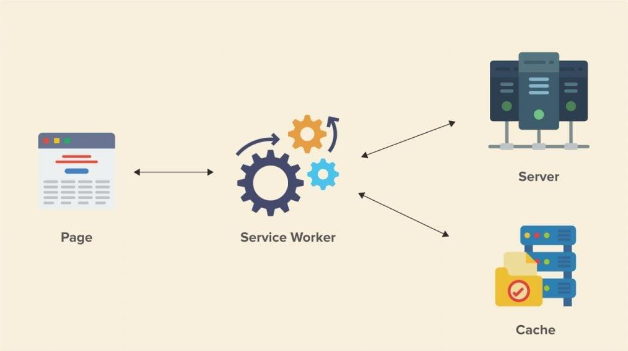
\includegraphics[width=0.5\textwidth]{serviceworker.png}
      \caption{Service worker diagram.}
    \end{figure}

    \paragraph{Service workers have emerged as a transformative PWA technology in the realm of web development, serving as a linchpin in the creation of Progressive Web Apps (PWAs) and enhancing the capabilities of websites in remarkable ways. Their advent represents a quantum leap in how developers can build offline-first experiences, ensuring that applications remain performant and reliable even in conditions of unreliable or absent connectivity.}
    
    \paragraph{At their core, service workers are essentially scripts that run in the background, separate from the web page itself. They operate in a context that’s distinct from the main browser thread, which means they don’t have direct access to the DOM. This separation is deliberate and advantageous, as it ensures that service workers don’t block or interfere with user interactions on the main thread, preserving the responsiveness and fluidity of web applications.}
    
    \paragraph{One of the primary features of service workers is their ability to intercept and control network requests. By doing so, they can cache assets and data, allowing for instant and offline access. }
    
    \paragraph{Service workers also play a crucial role in background data synchronization. For web apps that require data to be updated periodically, service workers can synchronize data in the background, ensuring that the user always has access to the latest information when they launch the application, even without an immediate internet connection.}

    \subsection{IndexedDB}

    \paragraph{IndexedDB is a low-level, NoSQL storage solution that’s built directly into modern web browsers. Unlike simpler storage solutions like local storage or session storage, which are limited to storing key-value pairs, IndexedDB offers the capability to store larger amounts of structured data, including files and blobs. Its ability to handle significant amounts of data, combined with its advanced search capabilities, makes it an indispensable tool for web applications that require more complex data operations on the client side.}
    
    \paragraph{Being asynchronous by nature, IndexedDB operations don’t block the main application thread. This ensures that even intensive data operations don’t hinder the responsiveness or performance of web applications. It’s a key aspect that aids in maintaining smooth user experiences, even in data-heavy applications.}
    
    \paragraph{Transactions are another vital feature of IndexedDB. They ensure data integrity by allowing multiple operations to be grouped together. If one operation within a transaction fails, the entire transaction can be rolled back, ensuring that the database remains in a consistent state.}

    \subsection{Background Sync API}

    \paragraph{The Background Sync API stands as a testament to the advancements in web development, specifically aimed at improving the user experience in web applications, particularly in scenarios of intermittent connectivity. It bridges the gap between offline-first experiences and real-time updates, ensuring web applications are both reliable and fresh.}
    
    \paragraph{The primary function of the Background Sync API is to delay actions until a stable internet connection is established. This can be particularly useful for operations like posting a blog comment, submitting a form, or updating user settings. If a user performs such an operation while offline or in a shaky connection environment, instead of failing the request, the Background Sync API ensures that the action is completed once the connection is back.}
    
    \paragraph{One of the standout benefits of the Background Sync API is enhancing the user experience. By using this API, developers can ensure that users don’t encounter frustrating errors or have to remember to retry actions once they’re back online. It’s all handled seamlessly in the background.}
    
    \paragraph{Another significant advantage is its potential to conserve data and battery on mobile devices. Instead of repeatedly attempting and failing to perform actions due to a poor connection – which can drain battery and data – the Background Sync API ensures that actions are only attempted when they’re likely to succeed.}

    \section{Testing and Debugging PWA Development Tools}

    \paragraph{With the advanced capabilities come challenges in ensuring that PWAs work seamlessly across various devices, screen sizes, and network conditions. Fortunately, the developer community is equipped with a range of testing and debugging tools tailored for PWAs. Let’s delve into some of these tools and understand their significance.}

    \subsection{Chrome DevTools}

    \begin{figure}[h!]
      \centering
      
\includegraphics[width=0.5\textwidth]{devtools.png}
      \caption{Chrome DevTools logo.}
    \end{figure}
    
    \paragraph{Chrome DevTools, embedded within Google’s Chrome browser, is an indispensable suite of web development and debugging tools. Its comprehensive set of features allows developers to efficiently interact with, test, and debug web content in real-time. Over the years, it has evolved to be a vital part of a web developer’s workflow, transforming the process of web development into a more streamlined and insightful experience.}
    
    \paragraph{At its core, Chrome DevTools provides an interface to inspect and modify the DOM (Document Object Model) and CSS of a web page. This live editing capability allows developers to experiment with page layouts, tweak styles, and immediately see the effects of those changes. Such immediacy not only speeds up the development process but also fosters a deeper understanding of how web elements interact.}
    
    \paragraph{Beyond mere inspection, Chrome DevTools offers a robust Console for logging and executing JavaScript in the context of the inspected page. This console acts as both a playground and a diagnostic tool, enabling developers to test scripts and view any errors or logs generated by the web page’s scripts.}

    \subsection{Lighthouse}

    \begin{figure}[h!]
      \centering
      
\includegraphics[width=0.5\textwidth]{lighthouse.png}
      \caption{Google Lighthouse logo.}
    \end{figure}

    \paragraph{Lighthouse stands as one of the premier tools for developers aspiring to create top-tier web applications. Developed by Google, Lighthouse is an open-source, automated auditing tool tailored to help developers improve the quality of their web pages and web apps. In essence, it offers a beacon, guiding developers through the labyrinthine process of optimizing modern web experiences.}
    
    \paragraph{One of the standout features of Lighthouse is its comprehensiveness. When run against a web page, it doesn’t just look at one aspect but conducts a multi-faceted examination, spanning performance, accessibility, progressive web apps (PWAs), best practices, and SEO. Such breadth ensures that developers gain a well-rounded understanding of their application’s strengths and areas of improvement.}
    
    \paragraph{Performance optimization is a cornerstone of Lighthouse. By auditing metrics like First Contentful Paint, Time to Interactive, and Cumulative Layout Shift, Lighthouse offers insights into the user’s perception of speed and responsiveness. This is invaluable in today’s digital landscape, where user retention can heavily hinge on mere milliseconds of loading time.}

    \subsection{Cypress}

    \begin{figure}[h!]
      \centering
      
\includegraphics[width=0.5\textwidth]{cypress.png}
      \caption{Cypress logo.}
    \end{figure}

    \paragraph{Cypress is a front-end testing tool that developers and QA engineers alike have come to adore for its ease of use, powerful features, and intuitive design. Unlike some other testing tools that operate by running outside the browser and executing remote commands, Cypress runs directly inside the browser. This approach offers developers more control, better accuracy, and a clearer understanding of how the application behaves in a real-world scenario.}

    \paragraph{One of the hallmarks of Cypress is its real-time reloading capability. As you write tests, the platform automatically reloads and provides instant feedback, significantly reducing the feedback loop and enhancing productivity. This ‘live’ testing environment is particularly invaluable when debugging, allowing developers to see exactly what happens and when.}
    
    \paragraph{The Cypress Dashboard is another standout feature. It’s a sophisticated tool that provides insights into test runs, presenting visualizations of test status, progress, and performance. It even captures videos of test runs, allowing teams to review how tests are executed, which is extremely useful for troubleshooting failures in continuous integration (CI) environments.}
    
    \paragraph{Cypress is not just about testing individual units of code; it facilitates comprehensive testing of the entire user journey, from the first click to the final submission. Its API is designed to be both simple and expressive, enabling the creation of readable and maintainable test suites. Moreover, the tool integrates effortlessly with popular JavaScript frameworks like React, Vue, and Angular, making it versatile and adaptable to various project needs.}

    \section{Best Practices for Using PWA Development Tools}

    \paragraph{To successfully craft a PWA that not only appeals to users but also delivers outstanding performance, certain best practices need to be ingrained in the development process in addition to some best PWA development tools and technologies. Based on the provided outline, here are the recommended best practices:}

    \subsection{Offline-first Approach}

    \paragraph{One of the distinguishing features of PWAs is their ability to function even in the absence of a network connection. By adopting an offline-first approach, developers prioritize the availability of content and functionality, regardless of network conditions. Utilizing service workers and caching mechanisms, this strategy ensures that users can access the app’s essential features, enhancing reliability and user trust.}
    
    \subsection{Responsive Design and Mobile Optimization}

    \paragraph{In an age where users access content from a myriad of devices, from smartphones to desktops, a PWA must be adaptable. A responsive design ensures that the app looks and functions optimally across all screen sizes. Additionally, given the predominance of mobile devices, mobile optimization is crucial. This involves touch-friendly interfaces, efficient use of screen real estate, and intuitive navigation structures.}
    
    \subsection{Performance Optimization}

    \paragraph{A snappy and responsive PWA is more likely to retain users. Performance optimization encompasses several strategies, from minimizing and compressing assets and employing lazy loading, to using content delivery networks (CDNs). Every millisecond saved during load time can significantly enhance user engagement, reduce bounce rates, and improve the overall user experience.}
    
    \subsection{PWA Install Banners and Prompts}

    \paragraph{For a truly native-like experience, PWAs can be added to the device’s home screen. However, this feature is only as good as its discoverability. By implementing PWA install banners and prompts, developers can nudge users to install the app, making it easily accessible. These prompts should be non-intrusive and timed appropriately, offering users a clear value proposition for installation.}
    
    \subsection{Continuous Integration and Deployment (CI/CD) for PWAs}

    \paragraph{The web is dynamic, and PWAs need to evolve continuously to cater to changing user needs and technological advancements. By integrating CI/CD pipelines, developers can ensure that updates, features, and fixes are regularly and reliably pushed to the PWA. This not only ensures that users have access to the latest offerings but also that any potential issues are swiftly addressed, maintaining the integrity and reputation of the app.}


\clearpage

	\section{Bibliography}

    \begin{enumerate}
    
      \item Anh, D. T. (2023, 30 agosto). Top Best PWA development Tools and Technologies for your business. Magenest - One-Stop Digital Transformation Solution. 
      
      \href{https://magenest.com/en/pwa-development-tools/}{https://magenest.com/en/pwa-development-tools/}
      
    \end{enumerate}
	
	
\end{document}